\section{James}
This is the section dedicated to one of the team members (namely, James), and it was written individually. It includes a range of things; first subsection is a space for him to point out the strengths and weaknesses of the module, including complaints about the module coordinator Max Wilson. The second section has a selfie image with Max! The last part of it is the most important one. He has written a paragraph about what he has learned in this module. Though he could have written it in \textbf{Bold} or other fonts, he chose not to, for this would have taken longer, and he thought that the default styling worked well enough. 

Please do not forget:
\begin{itemize}
	\item First paragraph should have your comments about the module
	\item Second one, a selfie img with Max
	\item Last one, what you learned in this module.
\end{itemize}

\subsection{Comments about the module}
All in all, I've found the Software Fundamentals module to be an interesting one. In the past, I've done both a GCSE and an A Level in Computer Science, and I've also written a variety of small programs and scripts for the past 7\(\frac{1}{2}\) years or so. Whilst doing those courses, there were components that required we show the software engineering process, and although it was to a lesser extent, it still involved the main ideas of requirements and specifications, a prototype, development and testing. Being able to see how to properly do these things (as opposed to writing the documents without really knowing why I needed to) is actually really useful, and I'm almost certain that it will come in useful in next year's group project!

\subsection{Selfie with Max}

\begin{figure}[h]
\caption{Selfie with Max}
\centering
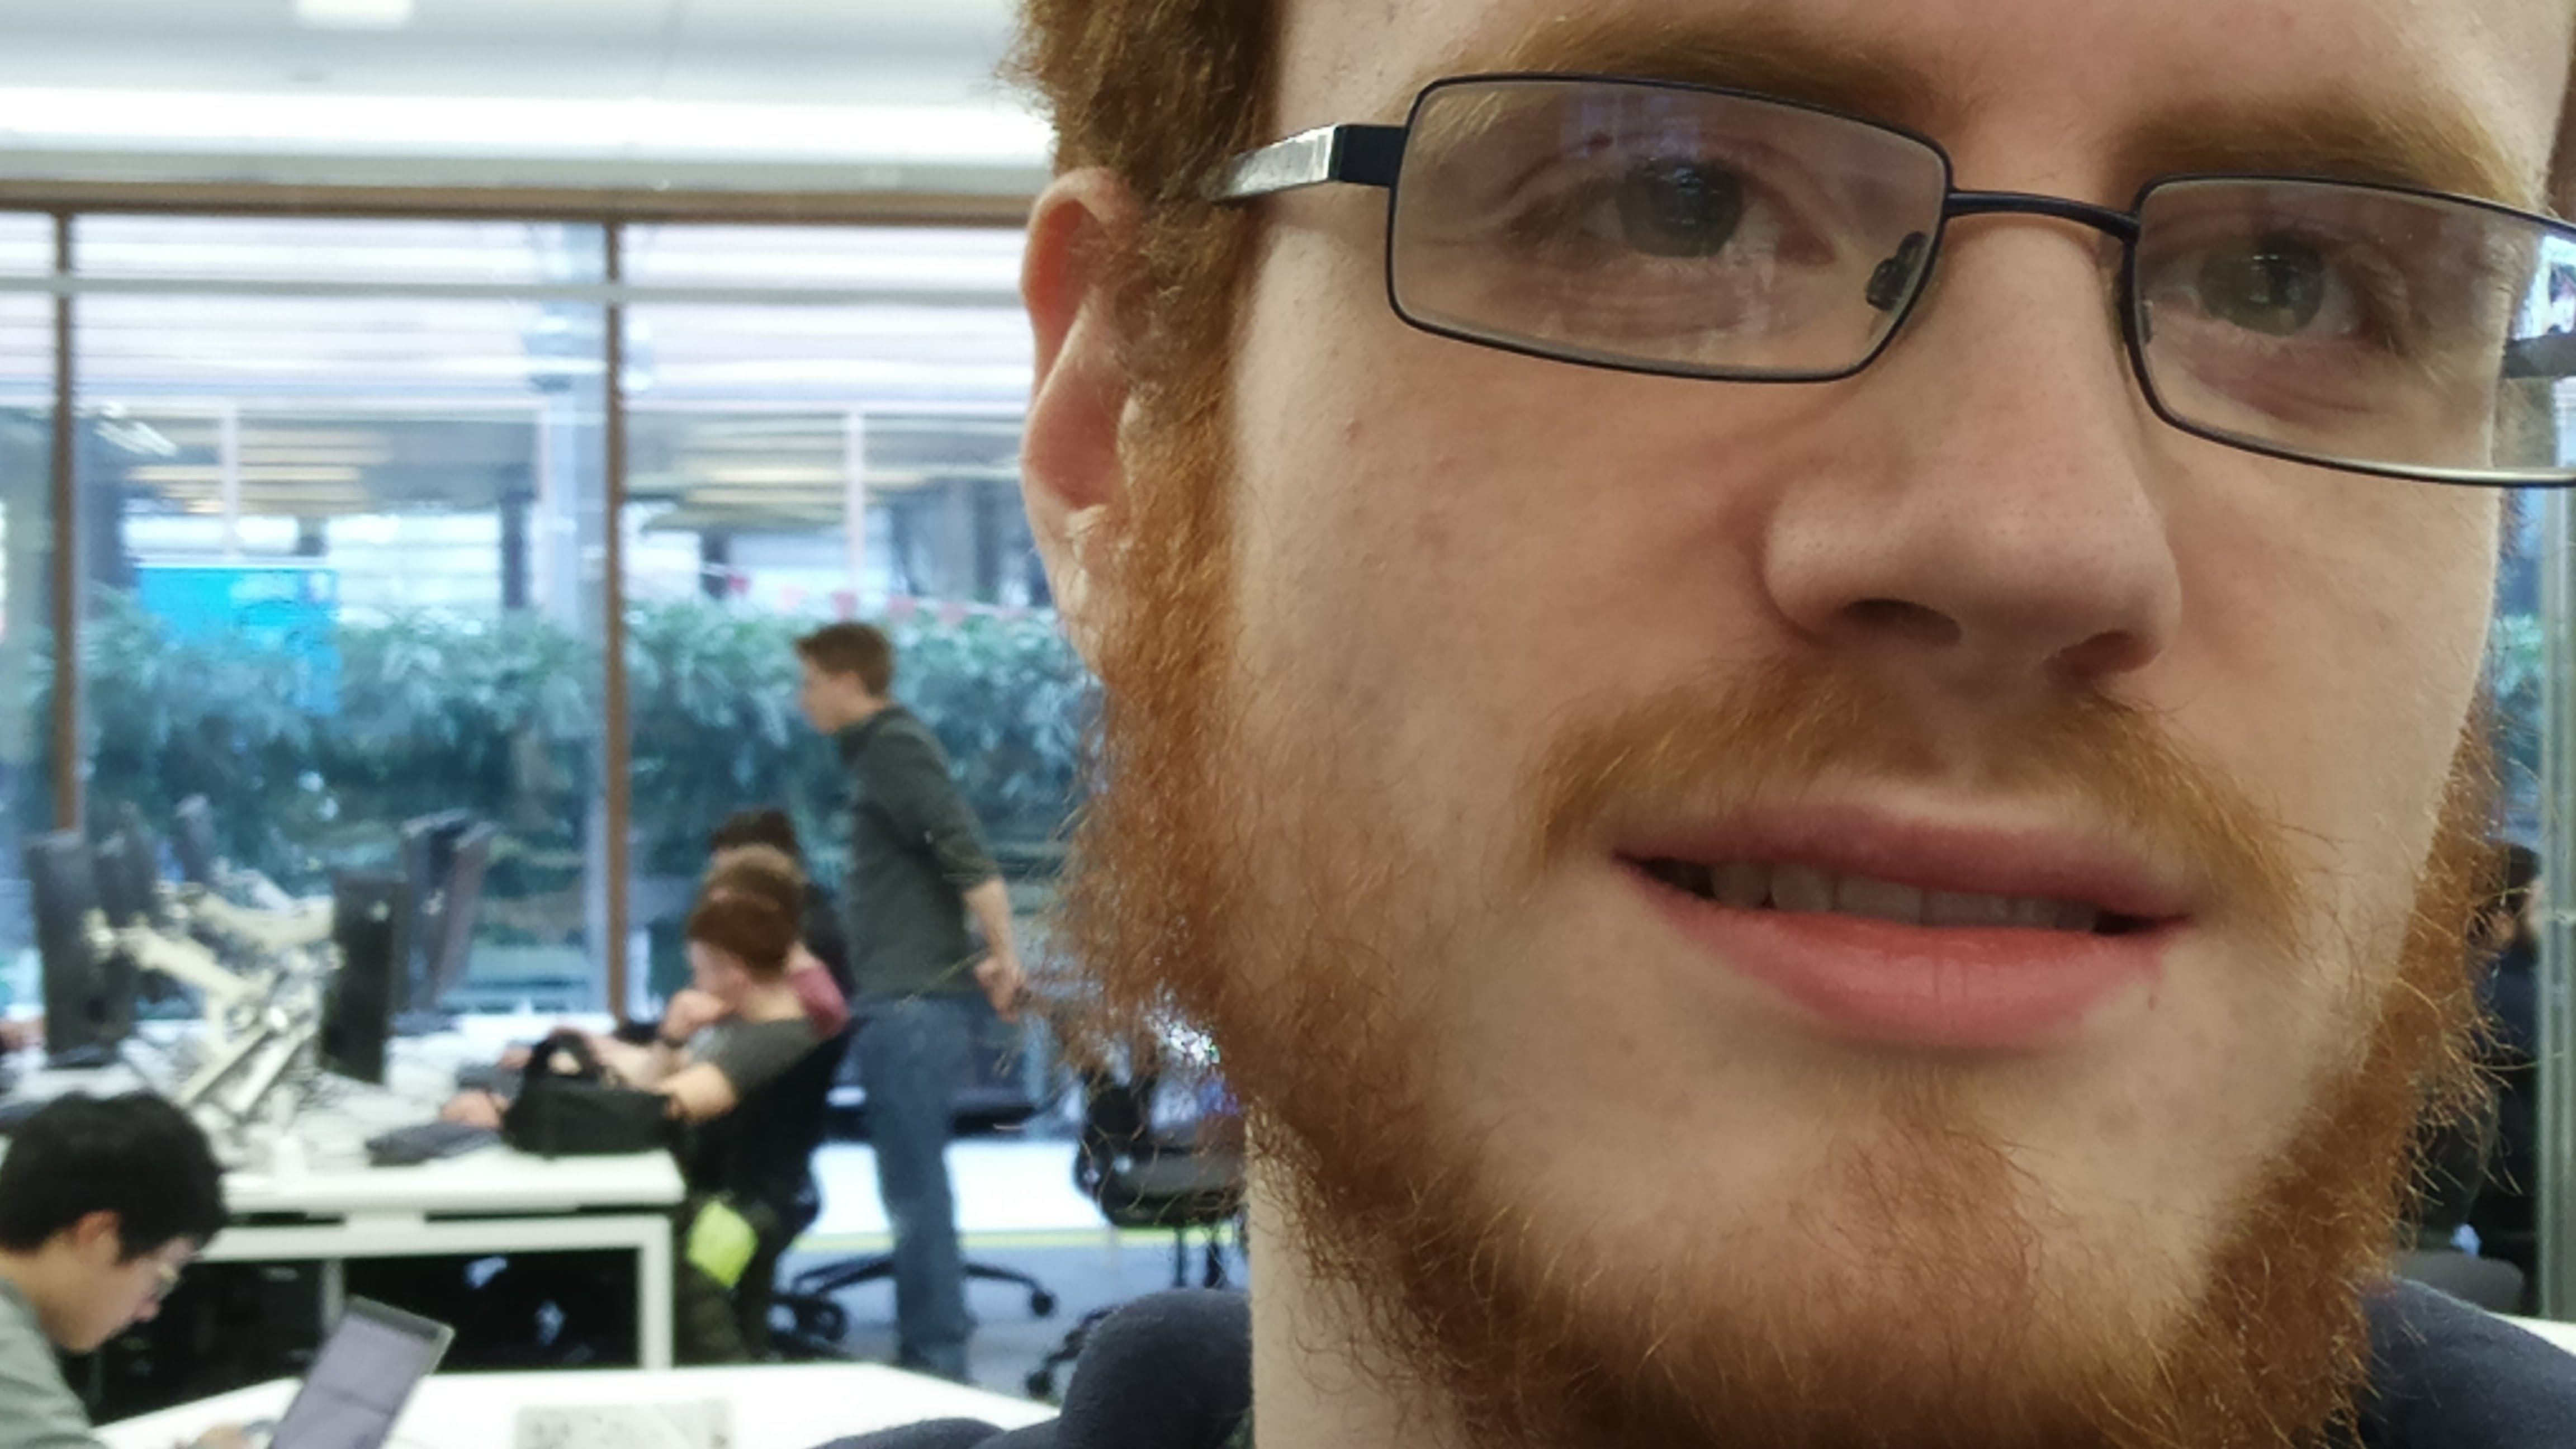
\includegraphics[width=0.5\textwidth]{images/MJCMAX.jpg}
\label{fig:jamesselfie}
\end{figure}

You can then use the label of the figure to reference it later with the command ${\backslash}ref$. you can comment out the next line to see an example of how it works.

My selfie with Max is in  Figure~\ref{fig:jamesselfie}.

\subsection{What I have learned in this module}
In this module, I've learned the process of developing software, from specifications and requirements to ongoing maintenance. Hopefully this module will allow me to have a better time working in a team next year in the group project, as we will not try to start by immediately writing code.